\documentclass[11pt]{article}

\usepackage[margin=1in]{geometry}
\usepackage{graphicx}
\usepackage{booktabs}
\usepackage{array}
\usepackage{xcolor}
\usepackage{amsmath}
\usepackage{siunitx}
\usepackage{caption}
\usepackage{enumitem}
\usepackage[hidelinks]{hyperref}
\usepackage{titlesec}

\graphicspath{{../results/figures/}}

\definecolor{ohnolog}{HTML}{1F6FB2}
\definecolor{ssd}{HTML}{B8500A}
\definecolor{accent}{HTML}{2E7D32}

\titleformat{\section}{\large\bfseries\color{ohnolog}}{\thesection}{0.6em}{}
\titleformat{\subsection}{\normalsize\bfseries}{\thesubsection}{0.6em}{}

\newcommand{\dcfour}{\texttt{dup\_class4}}
\newcommand{\dispoh}{\textcolor{ohnolog}{dispersed\_ohnolog}}
\newcommand{\clusoh}{\textcolor{ohnolog}{clustered\_cis\_ohnolog}}
\newcommand{\clusssd}{\textcolor{ssd}{clustered\_SSD\_tandem}}
\newcommand{\dispssd}{\textcolor{ssd}{dispersed\_SSD}}

\title{\vspace{-2.5em}\textbf{A duplication-provenance $\times$ genomic-arrangement\\
framework for paralogous transcription factors\\
in the human immune system}}
\author{iteration15 (human-only) --- ETS P01 genomics platform}
\date{2026-06-29}

\begin{document}
\maketitle
\vspace{-1.5em}

\begin{abstract}
\noindent
We classify every human paralogous transcription factor (TF) on a $2\times2$ of
\textbf{duplication provenance} (2R whole-genome-duplication ohnolog vs.\ small-scale
duplication, SSD) $\times$ \textbf{genomic arrangement} (clustered \emph{cis} vs.\
dispersed), after removing the silent KRAB-ZNF and HOX arrays that confounded earlier
analyses. Asking which of the four categories is enriched for cell-type \emph{identity}
markers versus cytokine-\emph{response} genes, we find a clean dissociation: enrichment
for lineage-identity markers is a specific property of \emph{dispersed} ohnologs and is
\emph{erased} by clustering (PBMC odds ratio, OR$=1.79$; spleen OR$=2.87$; within-ohnolog
clustered-vs-dispersed OR$\approx0.33$--$0.47$), whereas cytokine-response enrichment
tracks ohnolog \emph{provenance} and \emph{survives} clustering. Dosage analysis shows
buffering is not a category-level trait, but specific clustered neighbours diverge:
SSD tandems co-amplify (SAND/SP100 family, buffering index $B$ up to $1.84$) while a
\emph{cis}-ohnolog pair, STAT1/STAT4, is the cleanest buffer ($B=0.78$, partial
$r=-0.41$). We interpret clustering as an evolutionary mechanism that \emph{re-routes}
the regulatory potential of a 2R duplicate---from divergent lineage specialisation
toward a coordinated, dosage-coupled signalling-effector module, the configuration
exemplified by the ETS (ETS1/FLI1/ETS2/ERG) and STAT paralogons.
\end{abstract}

\section{Background and analytical framework}

Gene duplication is the raw material of regulatory innovation, but not all duplicates are
equivalent. Two axes matter. \textbf{Provenance:} a duplicate born in the two rounds of
vertebrate whole-genome duplication (2R-WGD, $\sim$500\,Mya)---an \emph{ohnolog}---is
dosage-balanced and preferentially retained, whereas a small-scale duplicate (SSD; tandem
or dispersed) is not. \textbf{Arrangement:} duplicates that remain in a genomic
\emph{cluster} share enhancers and topological context, while \emph{dispersed} copies sit
in independent regulatory landscapes. iteration15 crosses these into a single
four-category label, \dcfour:
{\footnotesize
\[
\begin{gathered}
\{\text{2R ohnolog},\ \text{SSD}\}\ \times\ \{\text{clustered \emph{cis}},\ \text{dispersed}\}\ \longrightarrow\\[2pt]
\{\dispoh,\ \clusoh,\ \clusssd,\ \dispssd\}.
\end{gathered}
\]}
A decisive control precedes the analysis: the KRAB-ZNF and HOX arrays---large, silent,
tandem-duplicated blocks shown previously to manufacture most of the raw
``clustered'' enrichment signal---are removed \emph{up front}, so every result below is
the KRAB/HOX-controlled effect.

\section{Methods (summary)}
Human TFs were curated from Lambert et al.\ (\textit{Cell} 2018); families were defined by
shared DNA-binding domain (DBD), with C2H2 zinc-fingers subdivided by HGNC accessory
domain (KRAB/SCAN/BTB) and CSD RNA-binders removed. Members were placed on hg38 (GENCODE
v45); KRAB-ZNF and HOX were excluded, and survivors were split into genomic clusters (two
same-family members adjacent iff no \emph{other} protein-coding gene lies between them)
versus singletons. Ohnolog provenance came from OHNOLOGS v2 plus a general
\emph{cis}-ohnolog rescue rule (any cluster containing $\geq1$ known ohnolog confers
ohnolog status on all members), which recovers the textbook FLI1/ERG pair with no hand
curation. Enrichment was tested per category by one-vs-rest Fisher exact tests (OR, 95\%
CI, BH-FDR) against the detectable paralogous-TF universe (catalog $\cap$ scRNA-seq
\texttt{var\_names}), with pairwise contrasts and a provenance$\times$arrangement
factorial logit. Dosage buffering used the Oesinghaus et al.\ (2025) human cytokine
dictionary: per within-family pair, buffering index $B=\mathrm{Var}(x{+}y)/(\mathrm{Var}\,x+\mathrm{Var}\,y)$
and a common-mode-removed partial correlation, benchmarked against a cross-family null.

\section{Part I--II: the four-category catalog}

After KRAB/HOX removal, 1{,}163 paralogous TFs survive, forming 78 genomic clusters
(184 clustered members) plus 979 singletons. Following pseudogene/readthrough cleanup, the
classified universe is \textbf{1{,}153 TFs} (Table~\ref{tab:counts}). The ETS quartet
(ETS1/FLI1/ETS2/ERG) and the STAT family (STAT1/3/4/5A/5B) fall in \clusoh; the chromosome-2
SAND cluster (SP100/110/140/140L), which contains no ohnolog member, remains \clusssd.

\begin{table}[h]
\centering
\caption{The four duplication categories ($n=1{,}153$ classified paralogous TFs).}
\label{tab:counts}
\begin{tabular}{lcl}
\toprule
\textbf{Category} & \textbf{$n$} & \textbf{Reference members} \\
\midrule
\dispoh   & 524 & scattered 2R-WGD singletons \\
\dispssd  & 450 & scattered small-scale duplicates \\
\clusoh   & 106 & \textbf{ETS1/FLI1/ETS2/ERG}, STAT1/3/4/5A/5B \\
\clusssd  & 73  & chr2 SAND: SP100/110/140/140L \\
\bottomrule
\end{tabular}
\end{table}

\section{Part III: identity vs.\ cytokine-response enrichment}

\subsection{Cell-type identity markers --- a property of \emph{dispersed} ohnologs}

In both human PBMC and spleen, \dispoh{} is the \emph{only} FDR-significant
identity-enriched group, and the two independent marker sets agree
(Table~\ref{tab:identity}, Figs.~\ref{fig:pbmc}--\ref{fig:spleen}). Clustering abolishes
the effect: within ohnologs, the clustered-vs-dispersed OR is $0.47$ (PBMC,
$p=0.008$) and $0.33$ (spleen, $p=0.008$); both clustered categories collapse to the SSD
background rate.

\begin{table}[h]
\centering
\footnotesize
\setlength{\tabcolsep}{5pt}
\caption{Identity-marker enrichment (one-vs-rest Fisher). FDR by Benjamini--Hochberg.}
\label{tab:identity}
\begin{tabular}{llS[table-format=1.3]S[table-format=1.2]S[table-format=1.4]l}
\toprule
\textbf{Tissue} & \textbf{Category} & {\textbf{rate}} & {\textbf{OR}} & {\textbf{FDR}} & \textbf{} \\
\midrule
PBMC   & \dispoh  & 0.287 & 1.79 & 0.0002  & enriched\,$\uparrow$ \\
PBMC   & \dispssd & 0.192 & 0.70 & 0.029   & depleted \\
PBMC   & \clusoh  & 0.160 & 0.61 & 0.119   & ns \\
PBMC   & \clusssd & 0.164 & 0.64 & 0.196   & ns \\
\midrule
Spleen & \dispoh  & 0.163 & 2.87 & {\num{7e-7}} & enriched\,$\uparrow$ \\
Spleen & \dispssd & 0.063 & 0.42 & 0.0001  & depleted \\
Spleen & \clusoh  & 0.061 & 0.51 & 0.169   & ns \\
Spleen & \clusssd & 0.070 & 0.60 & 0.331   & ns \\
\bottomrule
\end{tabular}
\end{table}

\begin{figure}[h]
\centering
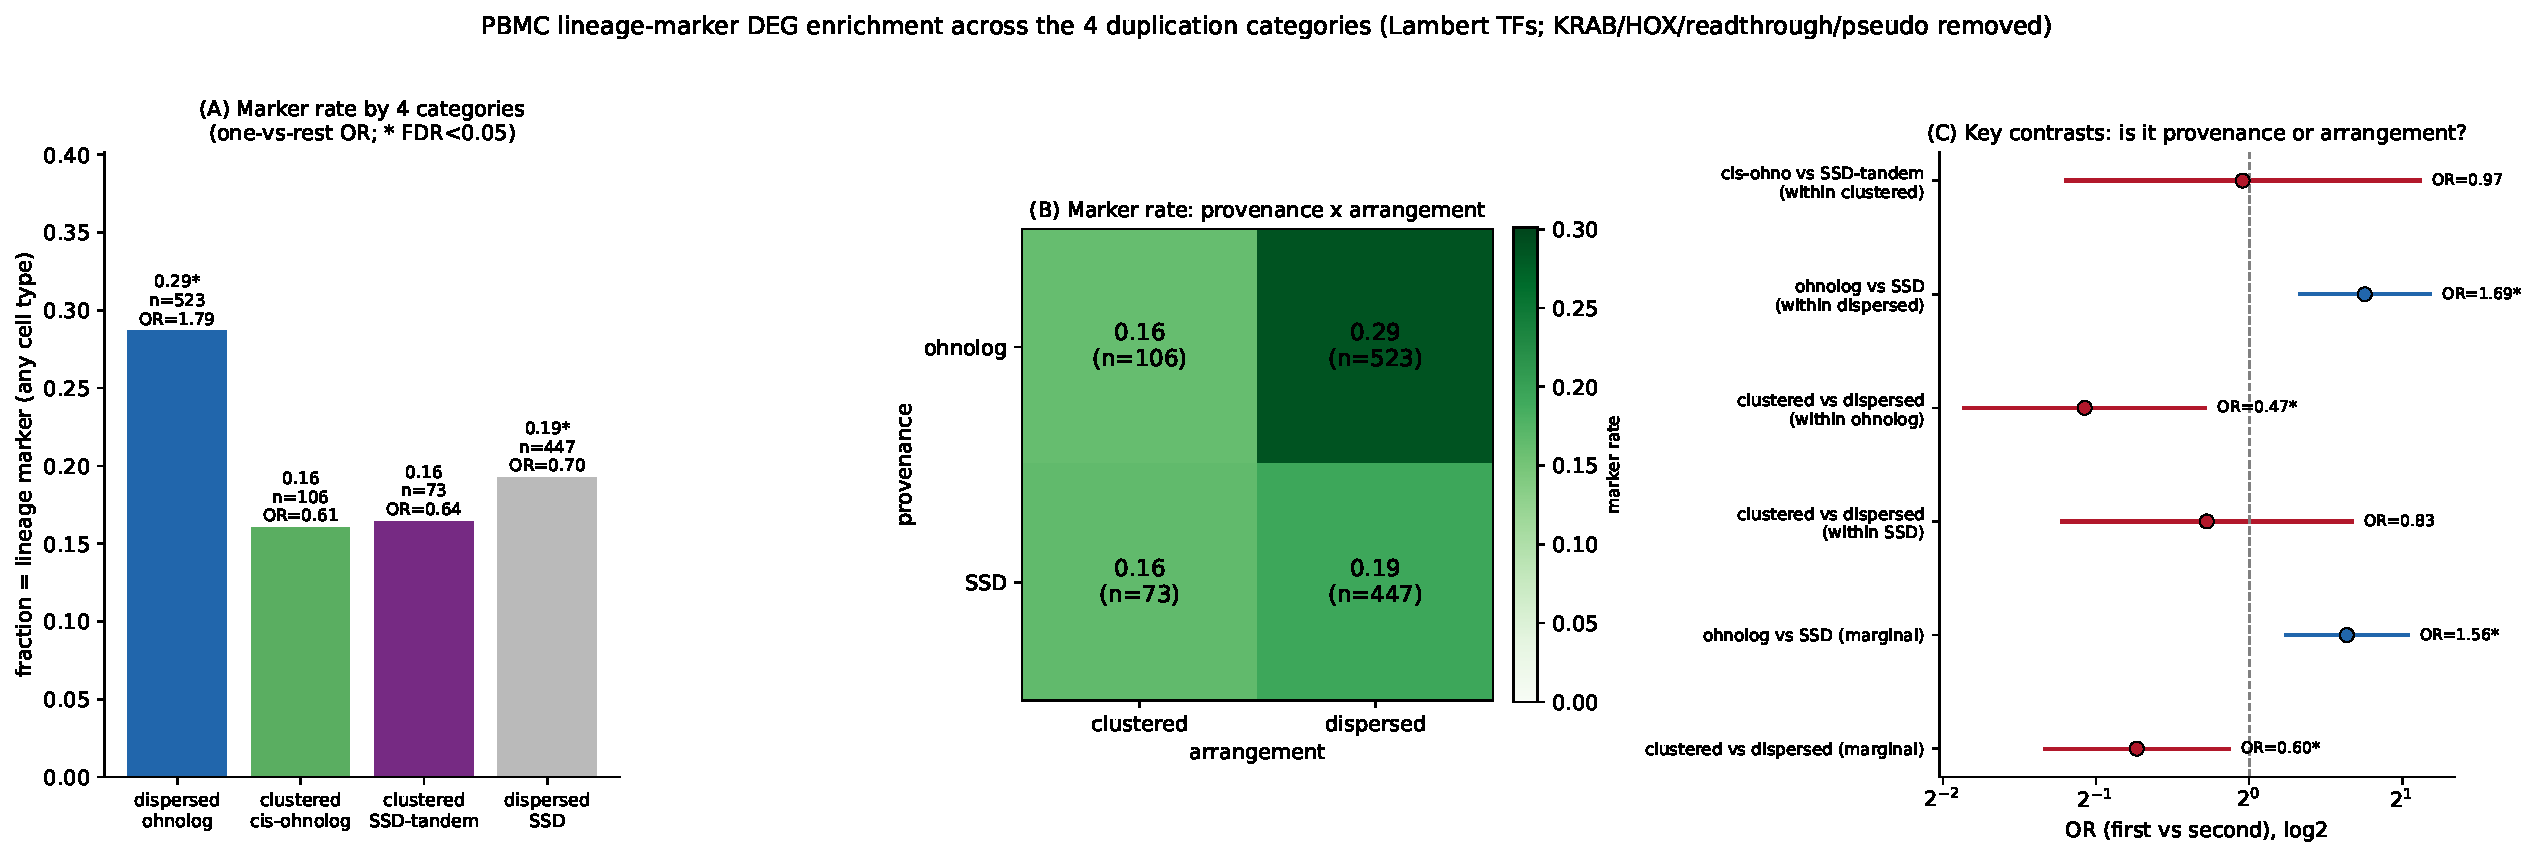
\includegraphics[width=0.82\textwidth]{TF_dup4_DEG_OR.pdf}
\caption{PBMC identity-marker enrichment across the four duplication categories.
\dispoh{} is the single enriched group.}
\label{fig:pbmc}
\end{figure}

\begin{figure}[h]
\centering
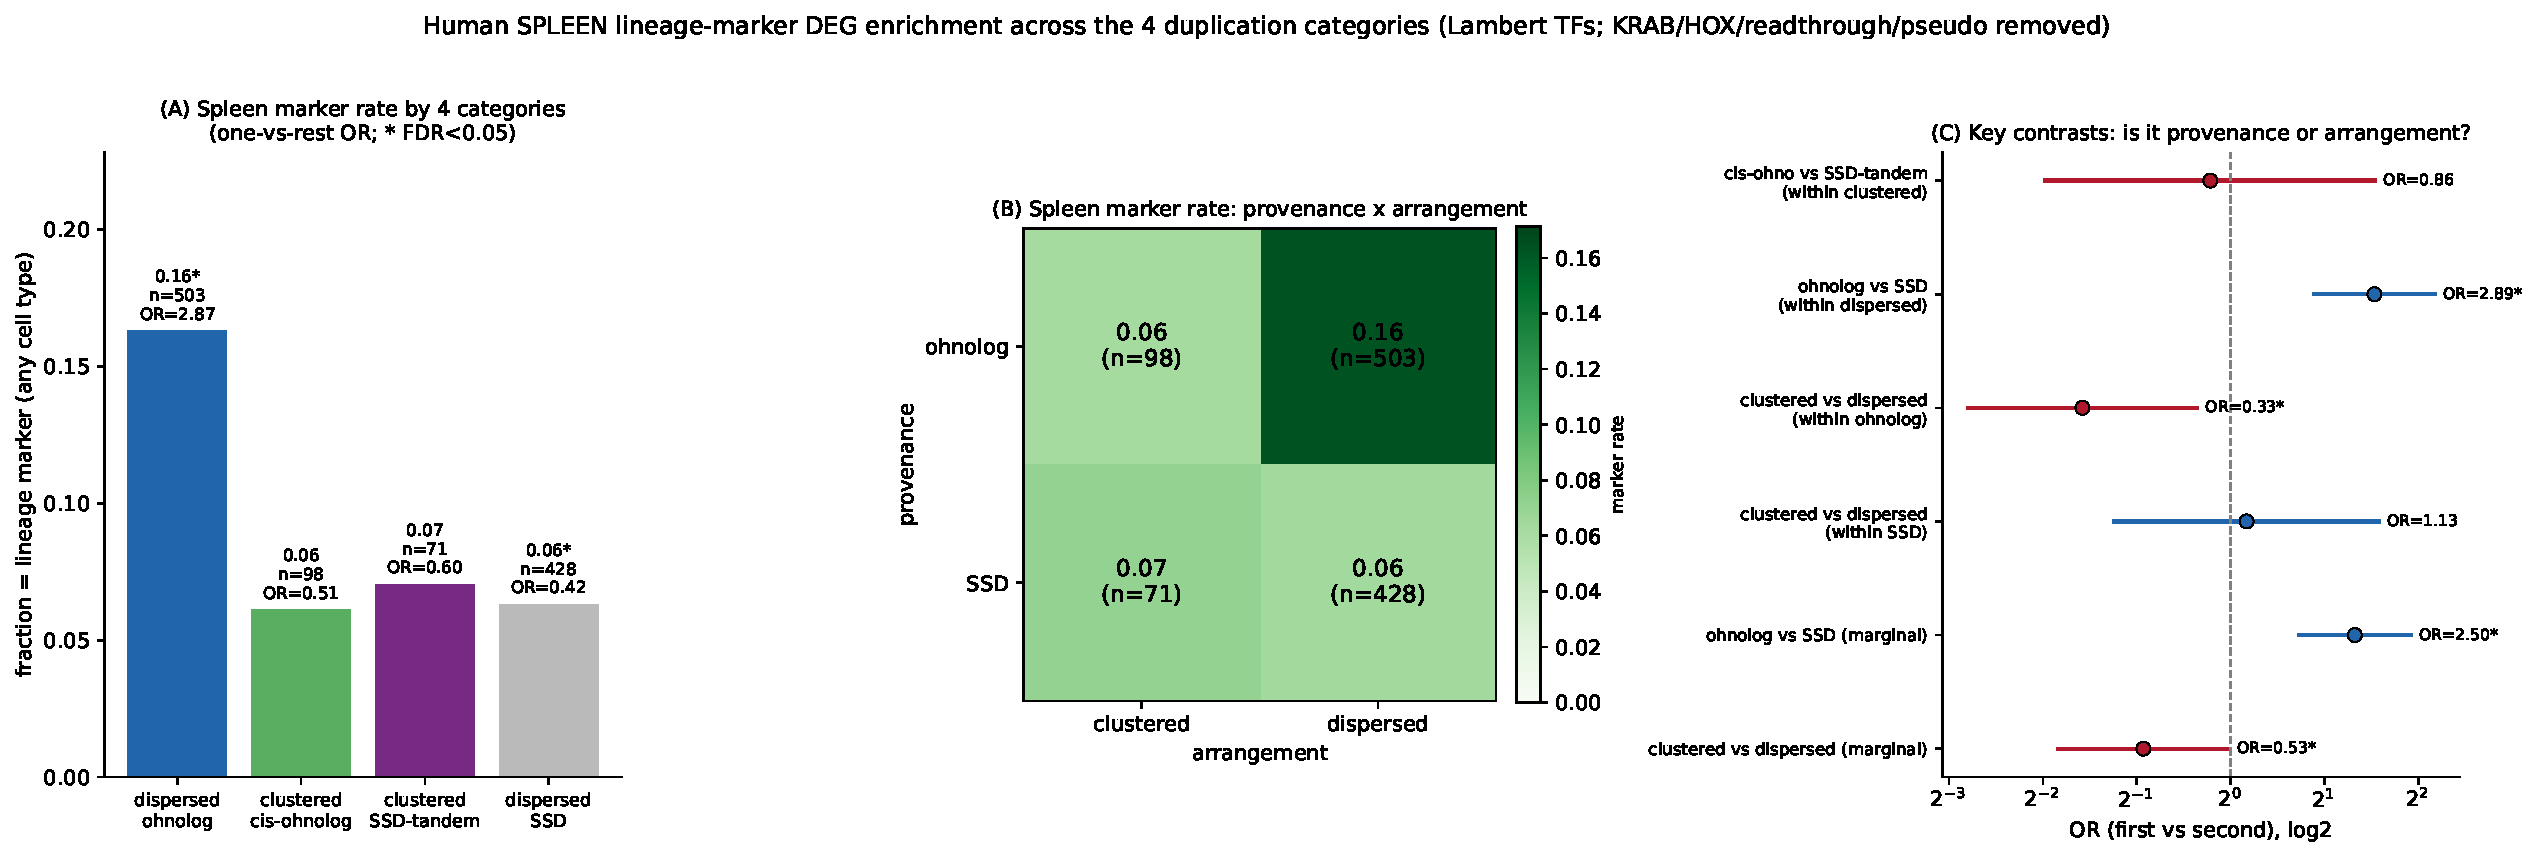
\includegraphics[width=0.82\textwidth]{TF_dup4_spleen_DEG_OR.pdf}
\caption{Spleen identity-marker enrichment (independent one-vs-rest markers) reproduces
the PBMC pattern: enrichment is exclusive to \dispoh.}
\label{fig:spleen}
\end{figure}

\subsection{Cytokine-response genes --- a property of ohnolog \emph{provenance} that survives clustering}

The cytokine-response picture dissociates sharply from identity
(Table~\ref{tab:cytokine}, Fig.~\ref{fig:cyto}). \dispoh{} is again most enriched
(rate $37.5\%$, OR$=1.67$, FDR$=2.3\times10^{-4}$), but \clusoh{} \emph{stays high}
(rate $29.2\%$, OR$=0.89$, $p=0.66$, i.e.\ not depleted), and the within-ohnolog
clustered-vs-dispersed contrast is \emph{not} significant ($p=0.12$)---unlike identity.
The provenance$\times$arrangement factorial confirms the asymmetry: the ohnolog main
effect is significant for all three readouts (PBMC adj-OR$=1.69$; spleen $2.89$; cytokine
$1.67$), the arrangement main effect and interaction are not.

\begin{table}[h]
\centering
\caption{Cytokine-response enrichment (one-vs-rest Fisher).}
\label{tab:cytokine}
\begin{tabular}{lS[table-format=1.3]S[table-format=1.2]S[table-format=1.4]l}
\toprule
\textbf{Category} & {\textbf{rate}} & {\textbf{OR}} & {\textbf{FDR}} & \textbf{} \\
\midrule
\dispoh  & 0.375 & 1.67 & 0.0002 & enriched\,$\uparrow$ \\
\clusoh  & 0.292 & 0.89 & 0.661  & retained (ns) \\
\dispssd & 0.264 & 0.68 & 0.007  & depleted \\
\clusssd & 0.219 & 0.59 & 0.119  & ns \\
\bottomrule
\end{tabular}
\end{table}

\begin{figure}[h]
\centering
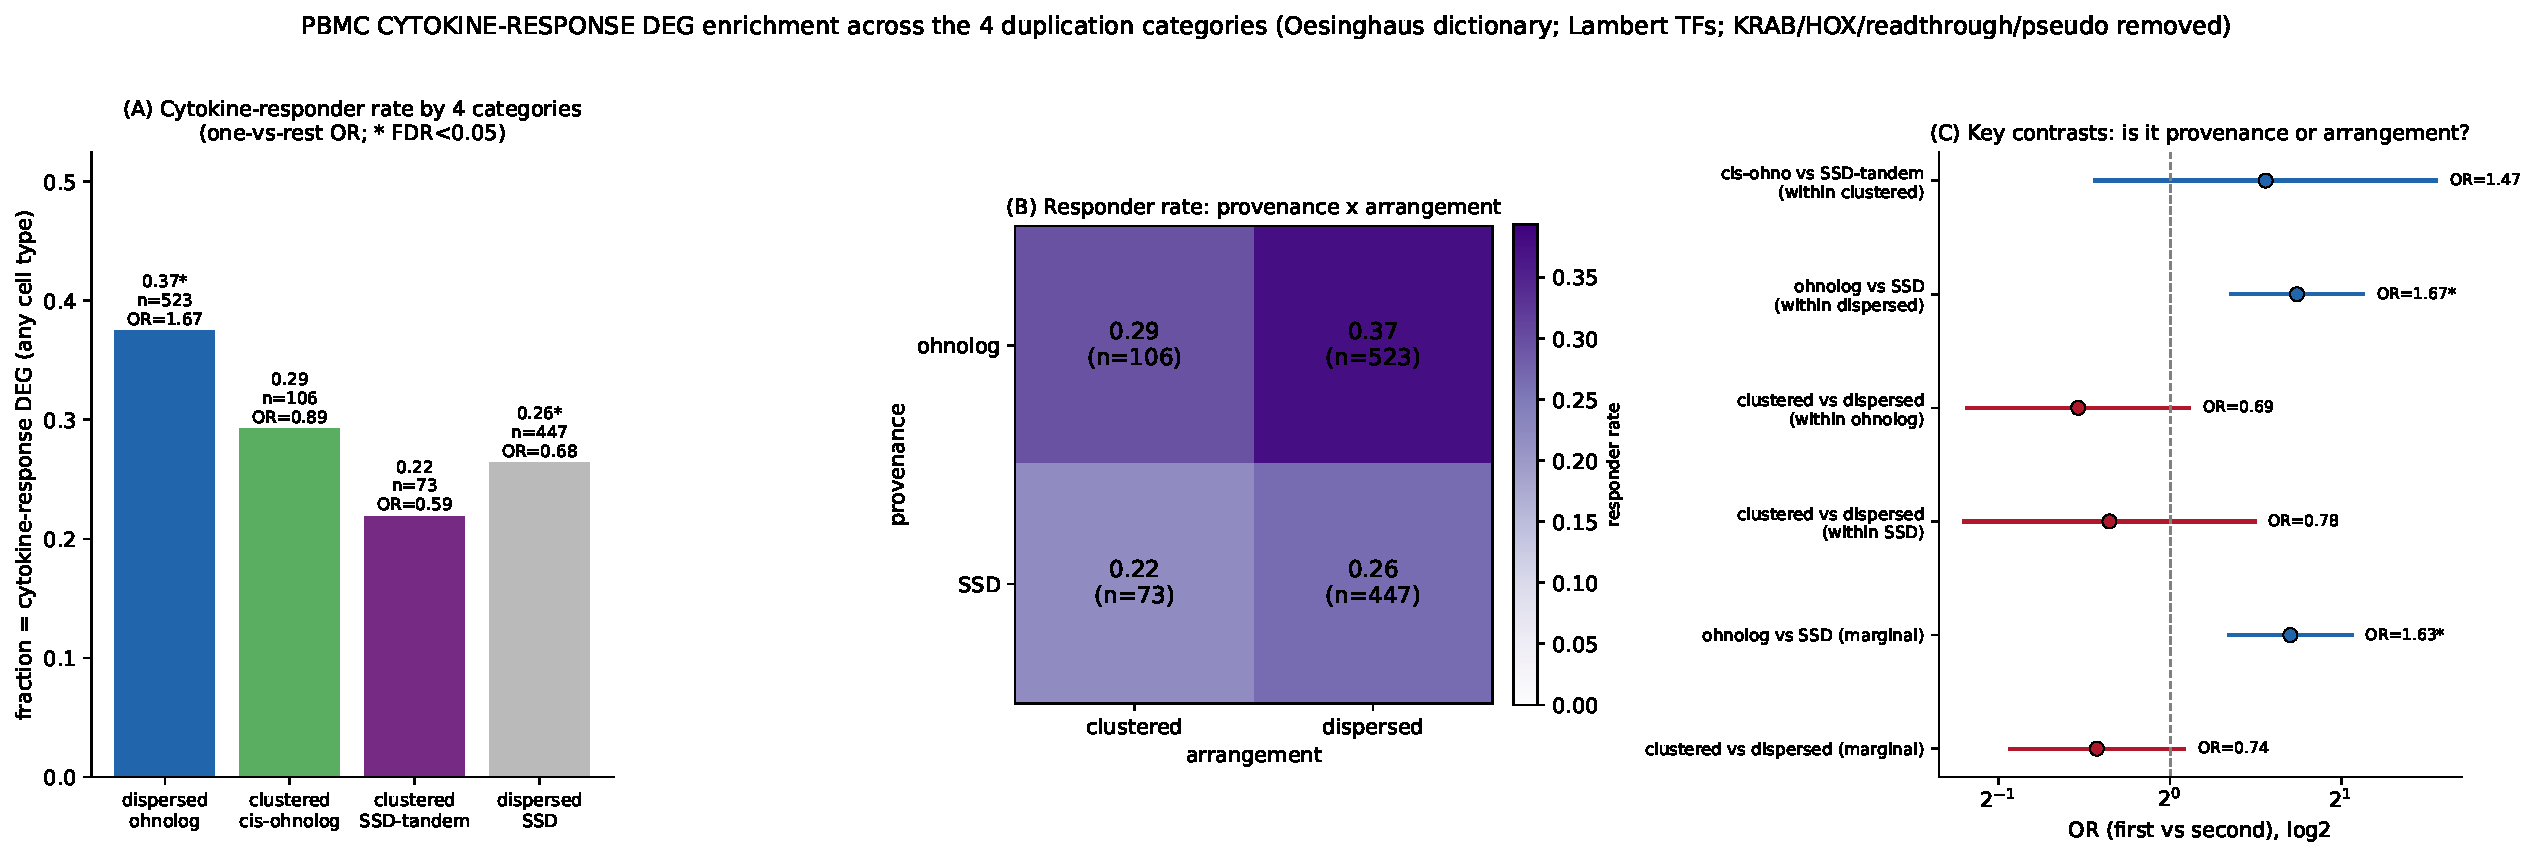
\includegraphics[width=0.82\textwidth]{TF_dup4_cytokine_DEG_OR.pdf}
\caption{Cytokine-response enrichment. Unlike identity, the clustered \emph{cis}-ohnolog
group does not collapse---clustering preserves the cytokine programme.}
\label{fig:cyto}
\end{figure}

\section{Part IV: dosage buffering by category}

Buffering is \emph{not} a category-level trait---every category's median $B\approx1.0$,
indistinguishable from the cross-family null (Kruskal--Wallis $p=0.14$;
Fig.~\ref{fig:buffer}). The signal lives in specific \emph{neighbour} pairs, where the two
clustered categories diverge (cis vs.\ SSD-tandem neighbour $B$ contrast $p=0.038$):

\begin{itemize}[leftmargin=1.4em,itemsep=2pt]
\item \textbf{SSD-tandem neighbours co-amplify.} The chr2 SAND/SP100 family shows
$B$ up to $1.84$ (SP100/SP110, partial $r=0.82$); all six SAND pairs have $B=1.4$--$1.8$
with strong positive partial correlation---redundant gene-dose stacking.
\item \textbf{A \emph{cis}-ohnolog pair is the cleanest buffer.} STAT1/STAT4 has $B=0.78$,
and common-mode removal flips its correlation negative ($r=-0.27\rightarrow$ partial
$r=-0.41$): active compensation, not shared drive.
\end{itemize}

\begin{figure}[h]
\centering
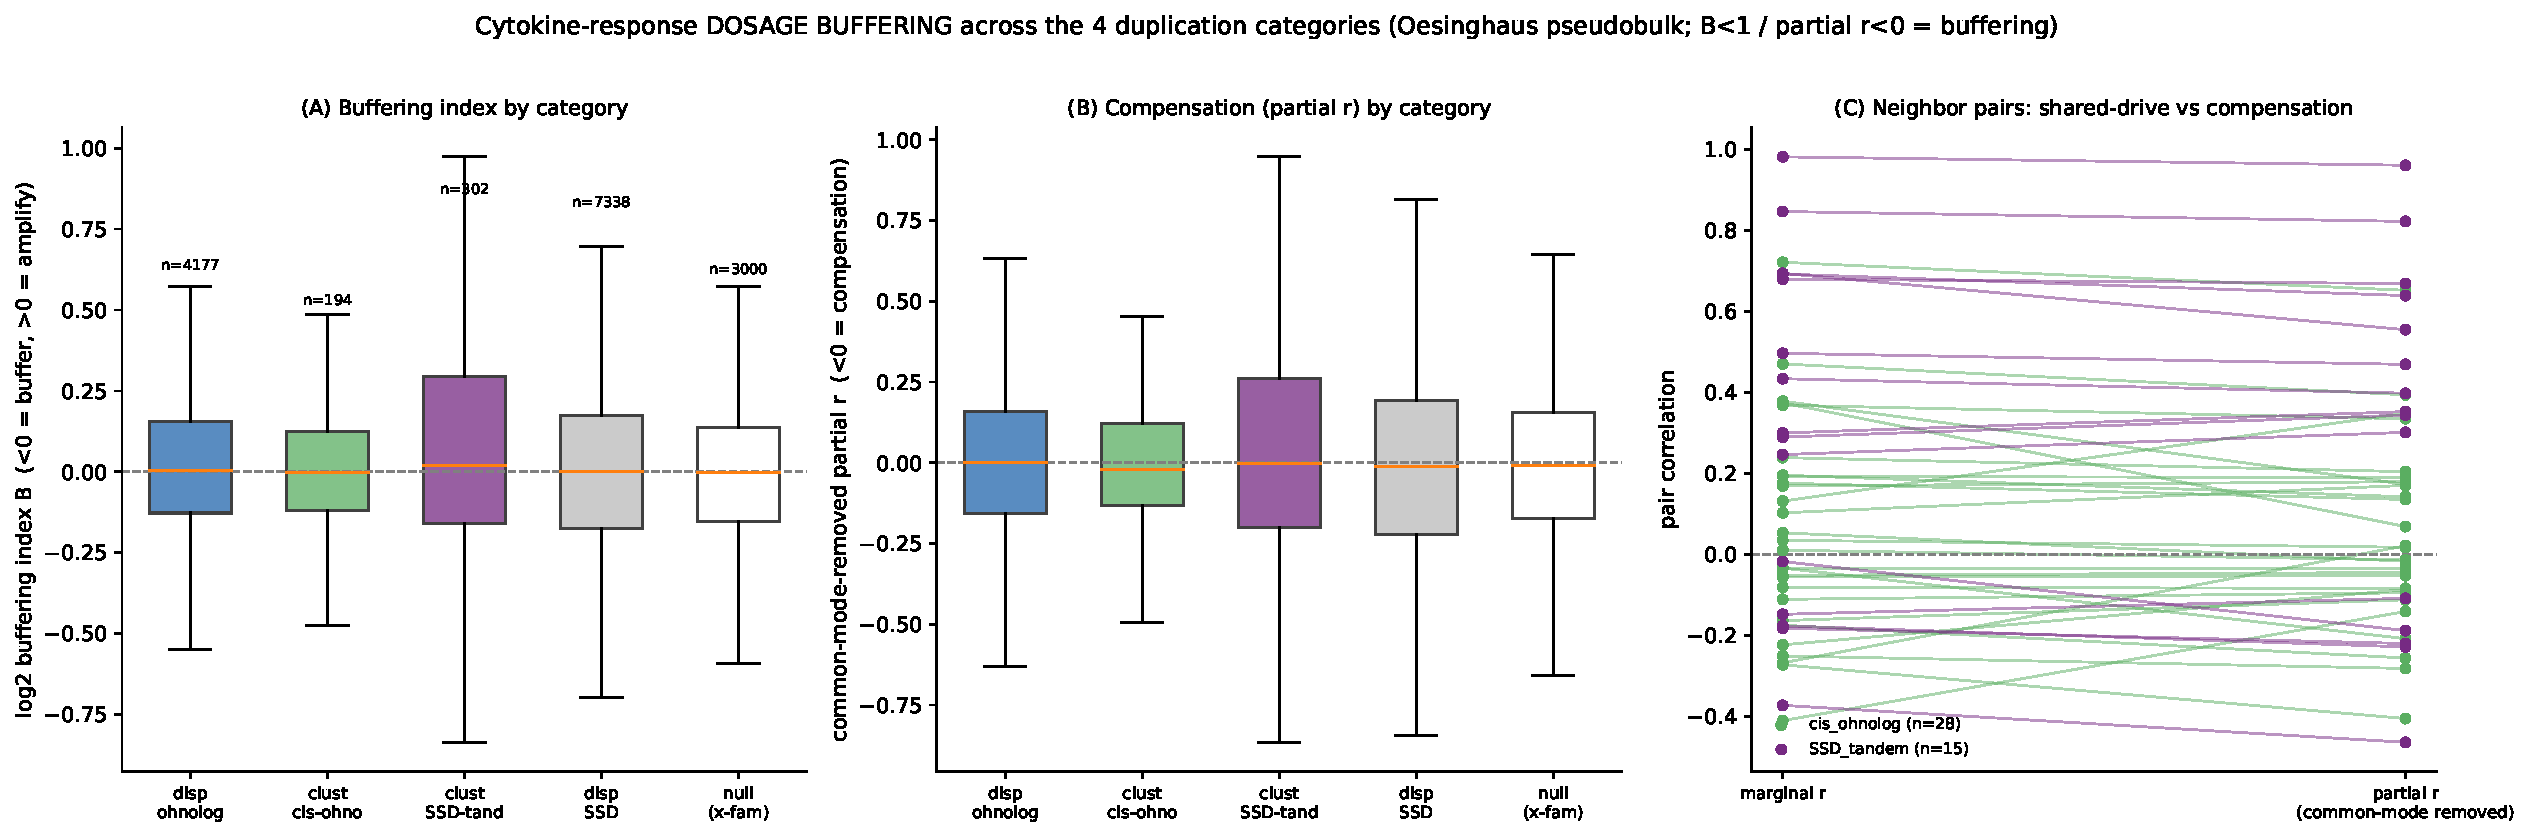
\includegraphics[width=0.86\textwidth]{cytokine_dosage_buffering_by_category.pdf}
\caption{Cytokine-dictionary dosage buffering by category. Category medians sit on the
null; divergence is a neighbour-level, pair-specific phenomenon (SAND amplification vs.\
STAT buffering).}
\label{fig:buffer}
\end{figure}

\section{Synthesis: what evolutionary advantage might clustering confer?}

The central result is a \textbf{dissociation}: \emph{provenance} (being a 2R ohnolog) sets
a duplicate's regulatory potential, but \emph{arrangement} (clustered vs.\ dispersed)
decides how that potential is spent. The two classical post-duplication fates---
\emph{neofunctionalisation} and \emph{dosage/sub-functional sharing}---map cleanly onto the
two arrangements, and clustering appears to carry several distinct selective advantages.

\paragraph{1. Dispersal buys divergence; clustering buys coordination.}
A dispersed ohnolog sits in its own regulatory landscape and is free to acquire
lineage-specific enhancers---hence \dispoh{} is the identity-TF reservoir. Clustering
removes that freedom: shared enhancers and a shared topological domain constrain the
copies to fire together. The advantage of \emph{losing} divergence is \textbf{guaranteed
co-regulation}: a cluster behaves as one regulatory unit, ensuring its members are
co-expressed in the right cell at the right time. This is exactly what we observe---
clustered ohnologs lose the (divergence-dependent) identity signal but \emph{retain} the
(coordination-dependent) cytokine-response signal.

\paragraph{2. Clustering converts an identity candidate into a signalling effector.}
The same \clusoh{} members that are \emph{not} enriched for identity markers \emph{are}
enriched (or at least not depleted) for cytokine-response genes. We read this as a
functional re-assignment: a 2R ohnolog that might otherwise have become a divergent
lineage-determining factor is instead recruited, as a coordinated block, into a
fast, signal-responsive effector programme. The ETS (ETS1/FLI1/ETS2/ERG) and STAT
paralogons---the engines of antigen-receptor and cytokine signalling---are the
archetypes. The selective advantage is a \textbf{ready-made, dosage-matched module} that
can be deployed coherently downstream of a signal.

\paragraph{3. Clustering enables paralog buffering at dosage-sensitive nodes.}
True compensatory buffering (STAT1/STAT4: partial $r=-0.41$) is found in a \emph{cis}-ohnolog
pair, consistent with the idea that physical proximity plus shared ancestry maintains
functional redundancy precisely where dosage matters. Buffering is selectively valuable
because it makes the network \textbf{robust to perturbation of a single member}: if one
paralog is lost or mutated, the neighbour compensates. This is the molecular basis for the
ETS P01 thesis---a paralog-buffered network whose phenotype on perturbation depends on how
much redundancy remains.

\paragraph{4. Clustering can also stack dose, not just buffer it.}
The SSD-tandem SAND/SP100 family shows the opposite neighbour behaviour---co-amplification
($B>1$). Here the advantage of physical clustering is \textbf{additive dosage}: tandem
copies of the same response amplify output, the simplest adaptive payoff of a local
duplication, with no regulatory rewiring. Thus clustering is not a single strategy; its
consequence (buffer vs.\ amplify) is itself gated by provenance (ohnolog vs.\ SSD).

\medskip\noindent
\textbf{In one sentence:} a 2R-WGD origin gives a TF pair the \emph{capacity} to become
either a divergent identity factor or a coordinated effector, and genomic clustering is the
switch---trading the evolvability of dispersal for the robustness and coordination of a
co-regulated, dosage-coupled module.

\section{Caveats}
\begin{enumerate}[leftmargin=1.6em,itemsep=1pt]
\item The OR denominator is the detectable paralogous-TF universe, not an
expression-matched background; the FDR-backed claims are the \dispoh{} identity
enrichment and the provenance factorial. The within-clustered contrasts rest on small
groups ($n\approx73$--$106$) and are trends.
\item Spleen cell-type labels derive from a blood-PBMC Azimuth transfer, so spleen is a
reproducibility contrast rather than added cell-type diversity; the cytokine dictionary is
also PBMC.
\item Provenance depends on the conservative OHNOLOGS v2; the \emph{cis}-ohnolog rescue
fixes only clustered misses (dispersed misses such as FEV stay SSD). The four-category
\dcfour{} label---not any per-gene mode---is the unit of analysis.
\end{enumerate}

\section{Conclusion}
Across human PBMC and spleen identity programmes and a PBMC cytokine dictionary, 2R-WGD
ohnolog \emph{provenance} is the determinant of a paralogous TF's regulatory enrichment,
while genomic \emph{arrangement} re-routes it: dispersal toward divergent cell-identity
roles, clustering toward coordinated, dosage-coupled cytokine effectors with the capacity
for paralog buffering. Clustering's evolutionary advantage is therefore not a single thing
but a trade---coordination, modular deployability and robustness in exchange for the
evolvability of independent divergence---and the ETS and STAT paralogons are its
clearest immune-system instantiations.

\end{document}
